\chapter{Simple Storage Service (S3)}\label{ch:simple-storage-service}

AWS S3 is a form of cloud-based object storage.
This is a style of network filesystem that treats each file as a separate object with a unique ID, which allows each
object to be served individually over a network with a single URL, which can also be enhanced with a content delivery
network~\parencite{amazon2022cloud}.

Each S3 instance is seperated into logical containers known as buckets.
Each S3 bucket can have its own credentials, its own endpoint and other permissions and configuration.
Object storage is particularly useful when creating an application that scales as you are billed per unit of storage
that you use, and in theory are able to use infinite storage as your application demands.
The only limitation with object storage is how much you are able to pay for.
Each object is automatically replicated across many nodes, providing data redundancy against multiple different
availability zones.

S3 is perhaps the most popular AWS service and used by many SaaS applications across the internet, for instance
Instagram, Facebook, Discord and Twitter are all known for using S3 or S3-style storage.
The advent of object storage has created an almost de-facto standard, which has lead for the creation of many
'S3-compatible' or 'S3-like' competitor solutions, such as those run by Google Cloud and Microsoft Azure.

\pagebreak
\section{Creating an S3 Bucket}\label{sec:creating-an-s3-bucket}

An important aspect of S3 is the encryption it provides.
When setting up S3 it can be specified whether or not to use a server-side encryption key.
Setting up an encryption key to be managed by AWS was the most secure option, so it was selected.

\begin{figure}[!htbp]
    \centering
    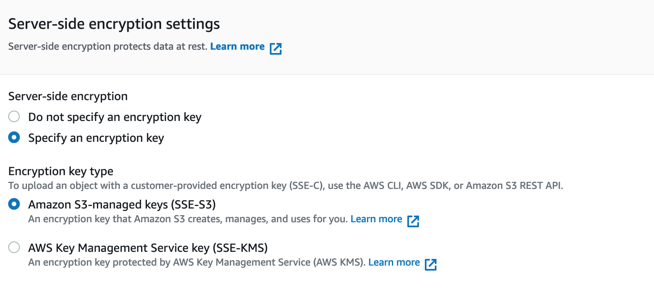
\includegraphics[width=\textwidth]{resources/s3/s3_encryption}
    \caption{Setting up the S3 encryption key.}
    \label{fig:s3-image-2}
\end{figure}

\begin{figure}[!htbp]
    \centering
    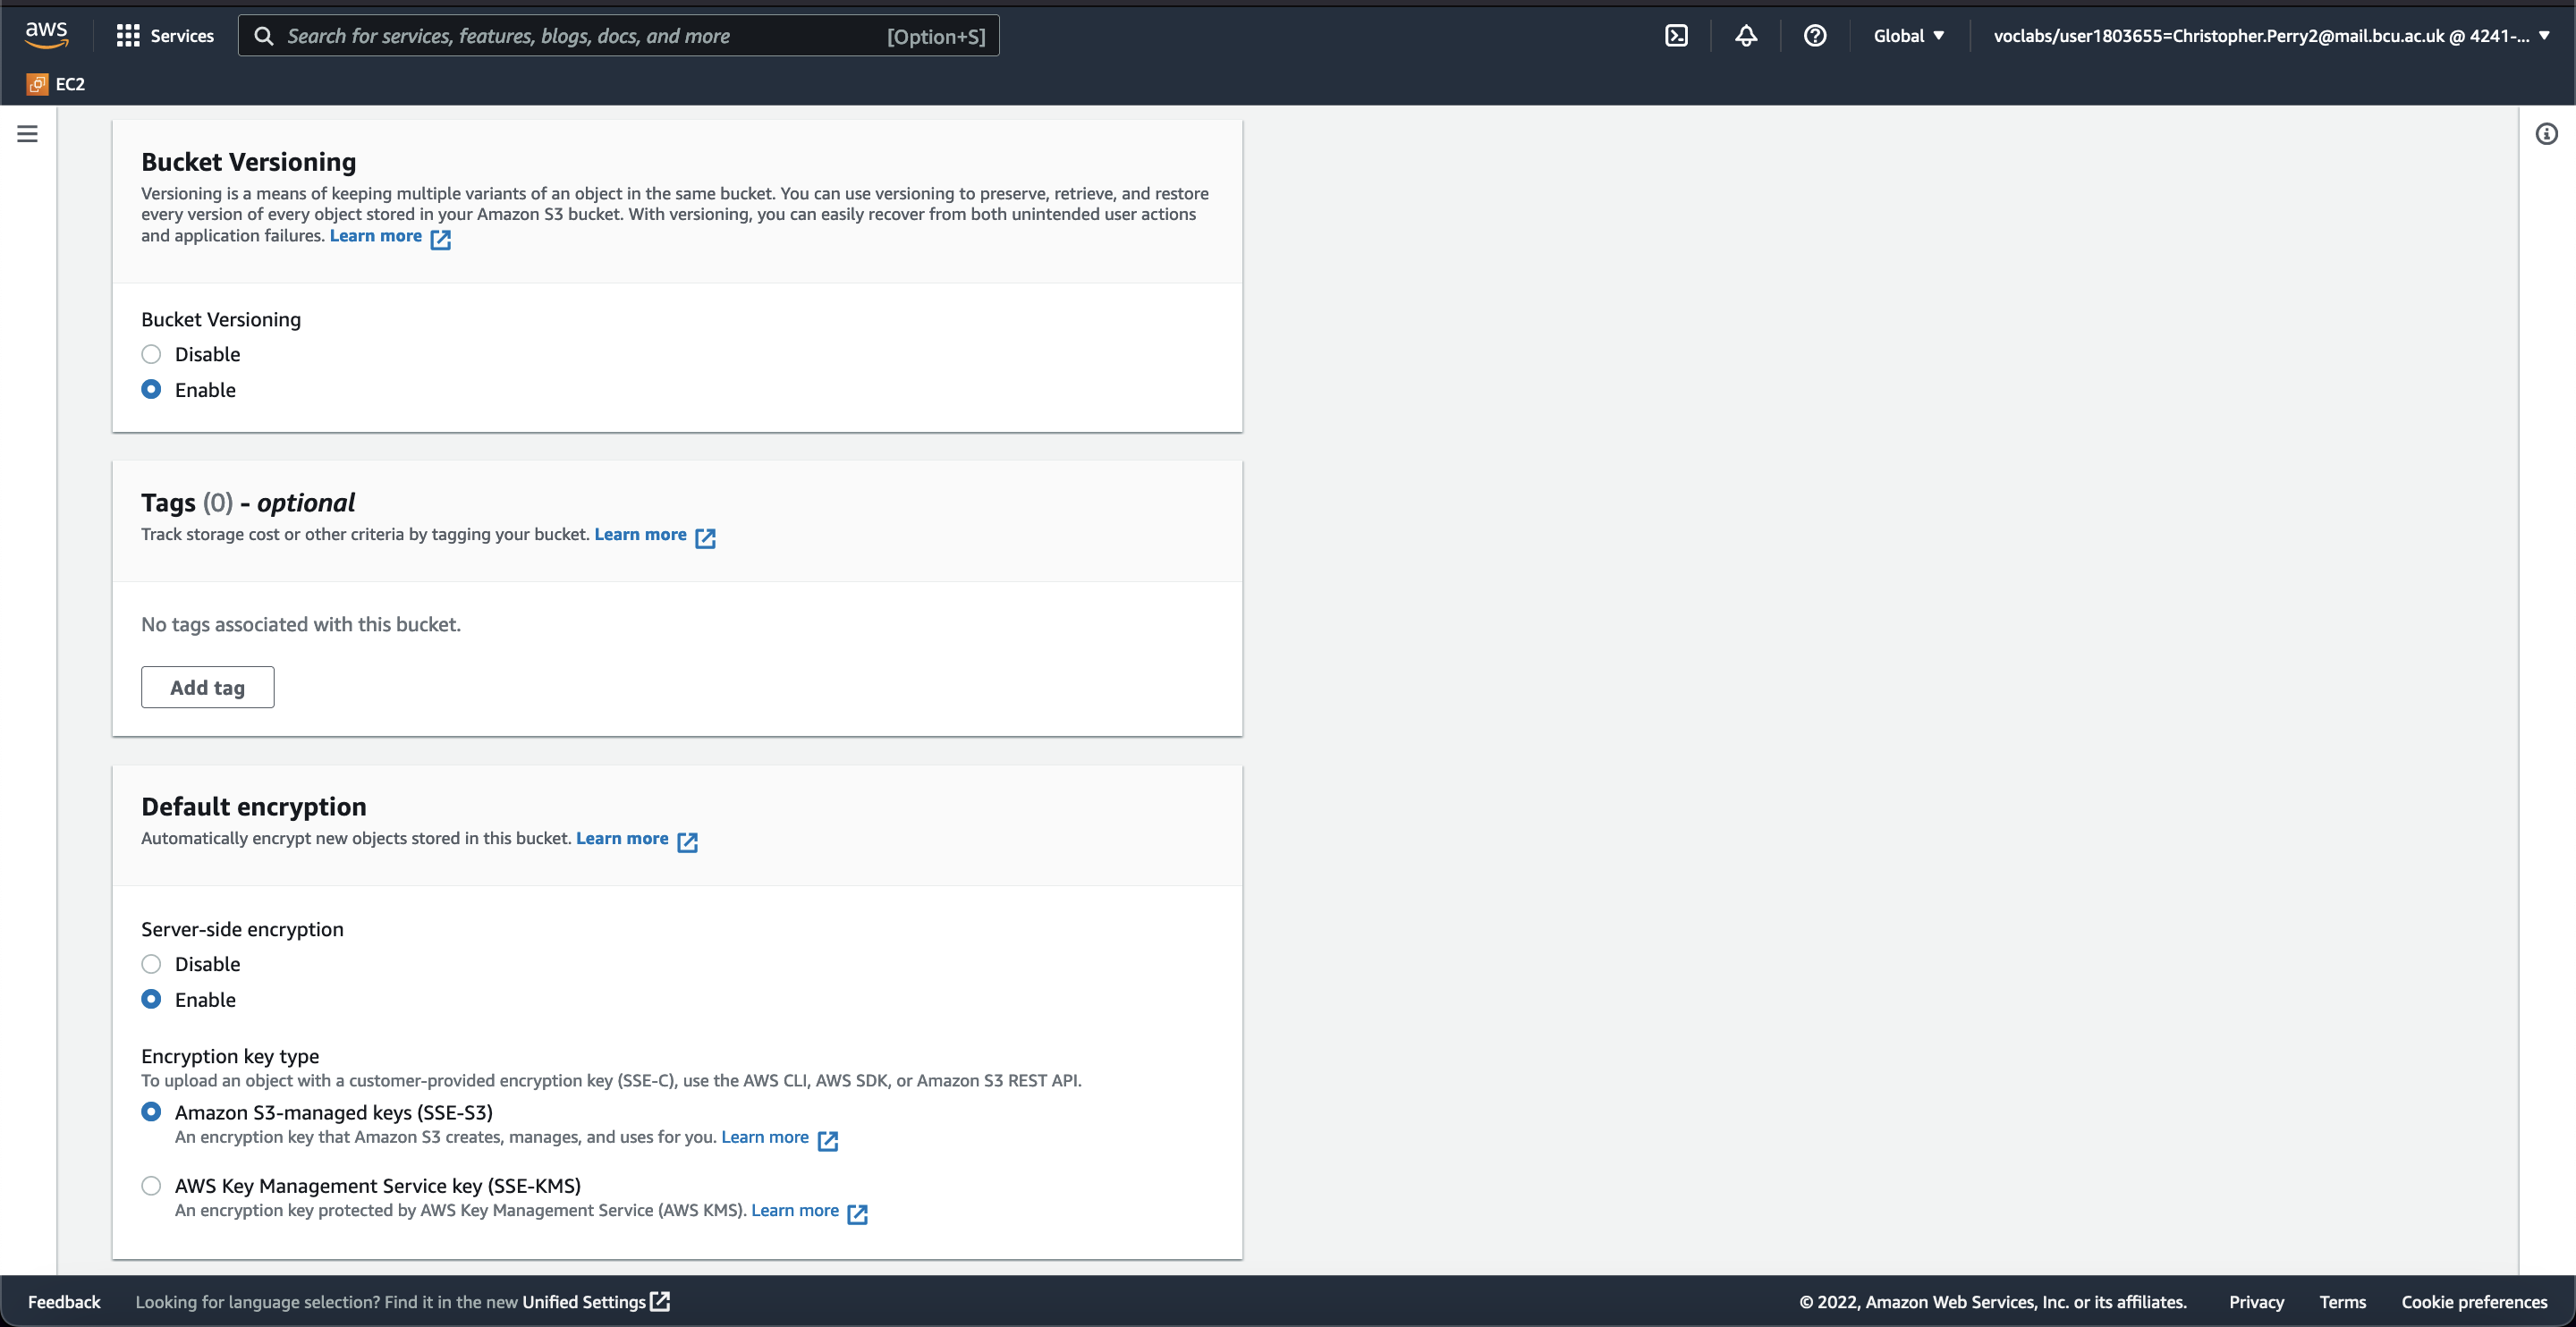
\includegraphics[width=\textwidth]{resources/s3/s3-versioning-encrypting}
    \caption{Setting up S3 versioning and encryption settings.}
    \label{fig:s3-versioning-encrypting}
\end{figure}

\pagebreak
When configuring an S3 bucket, the object ownership was must specified.
For setting object ownership, the recommended option was used.
This makes all of the images public, so fine-grain ACL control is not needed.

\begin{figure}[!htbp]
    \centering
    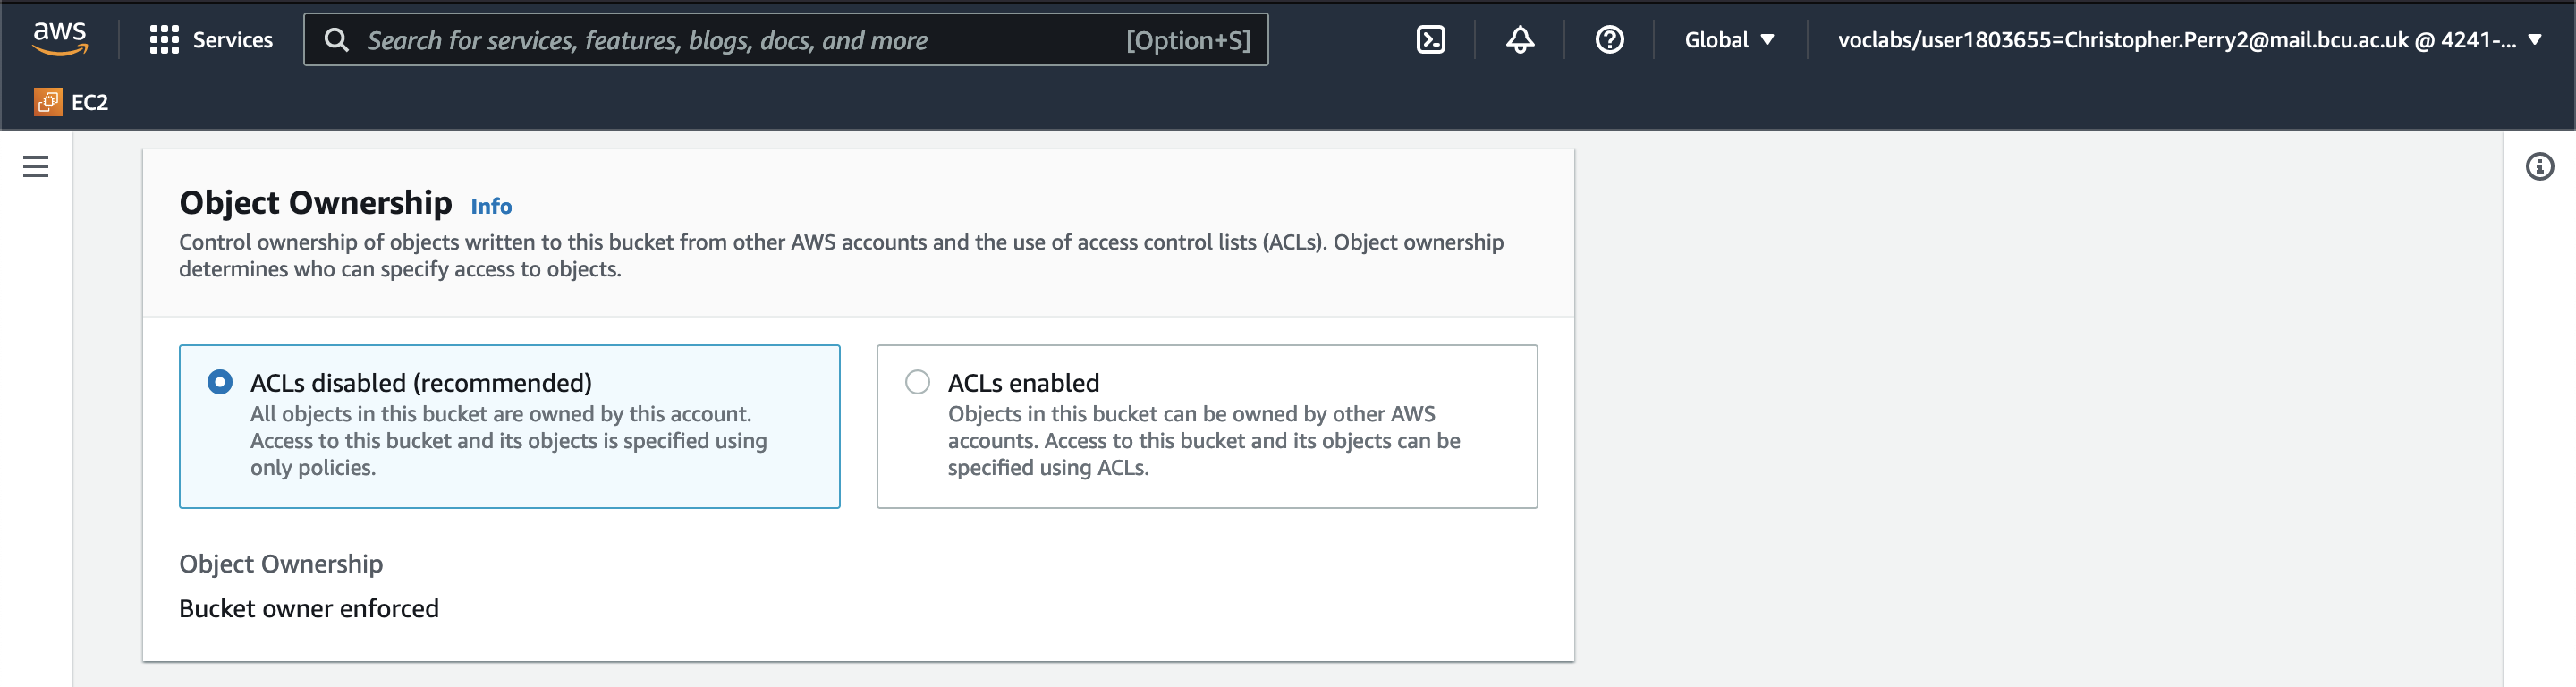
\includegraphics[width=125mm]{resources/s3/s3-object-ownership}
    \caption{Setting up S3 object ownership.}
    \label{fig:s3-object-ownership}
\end{figure}

Additionally, public read access to the S3 bucket was allowed, as all of the images are be public static assets and no
private assets are needed.

\begin{figure}[!htbp]
    \centering
    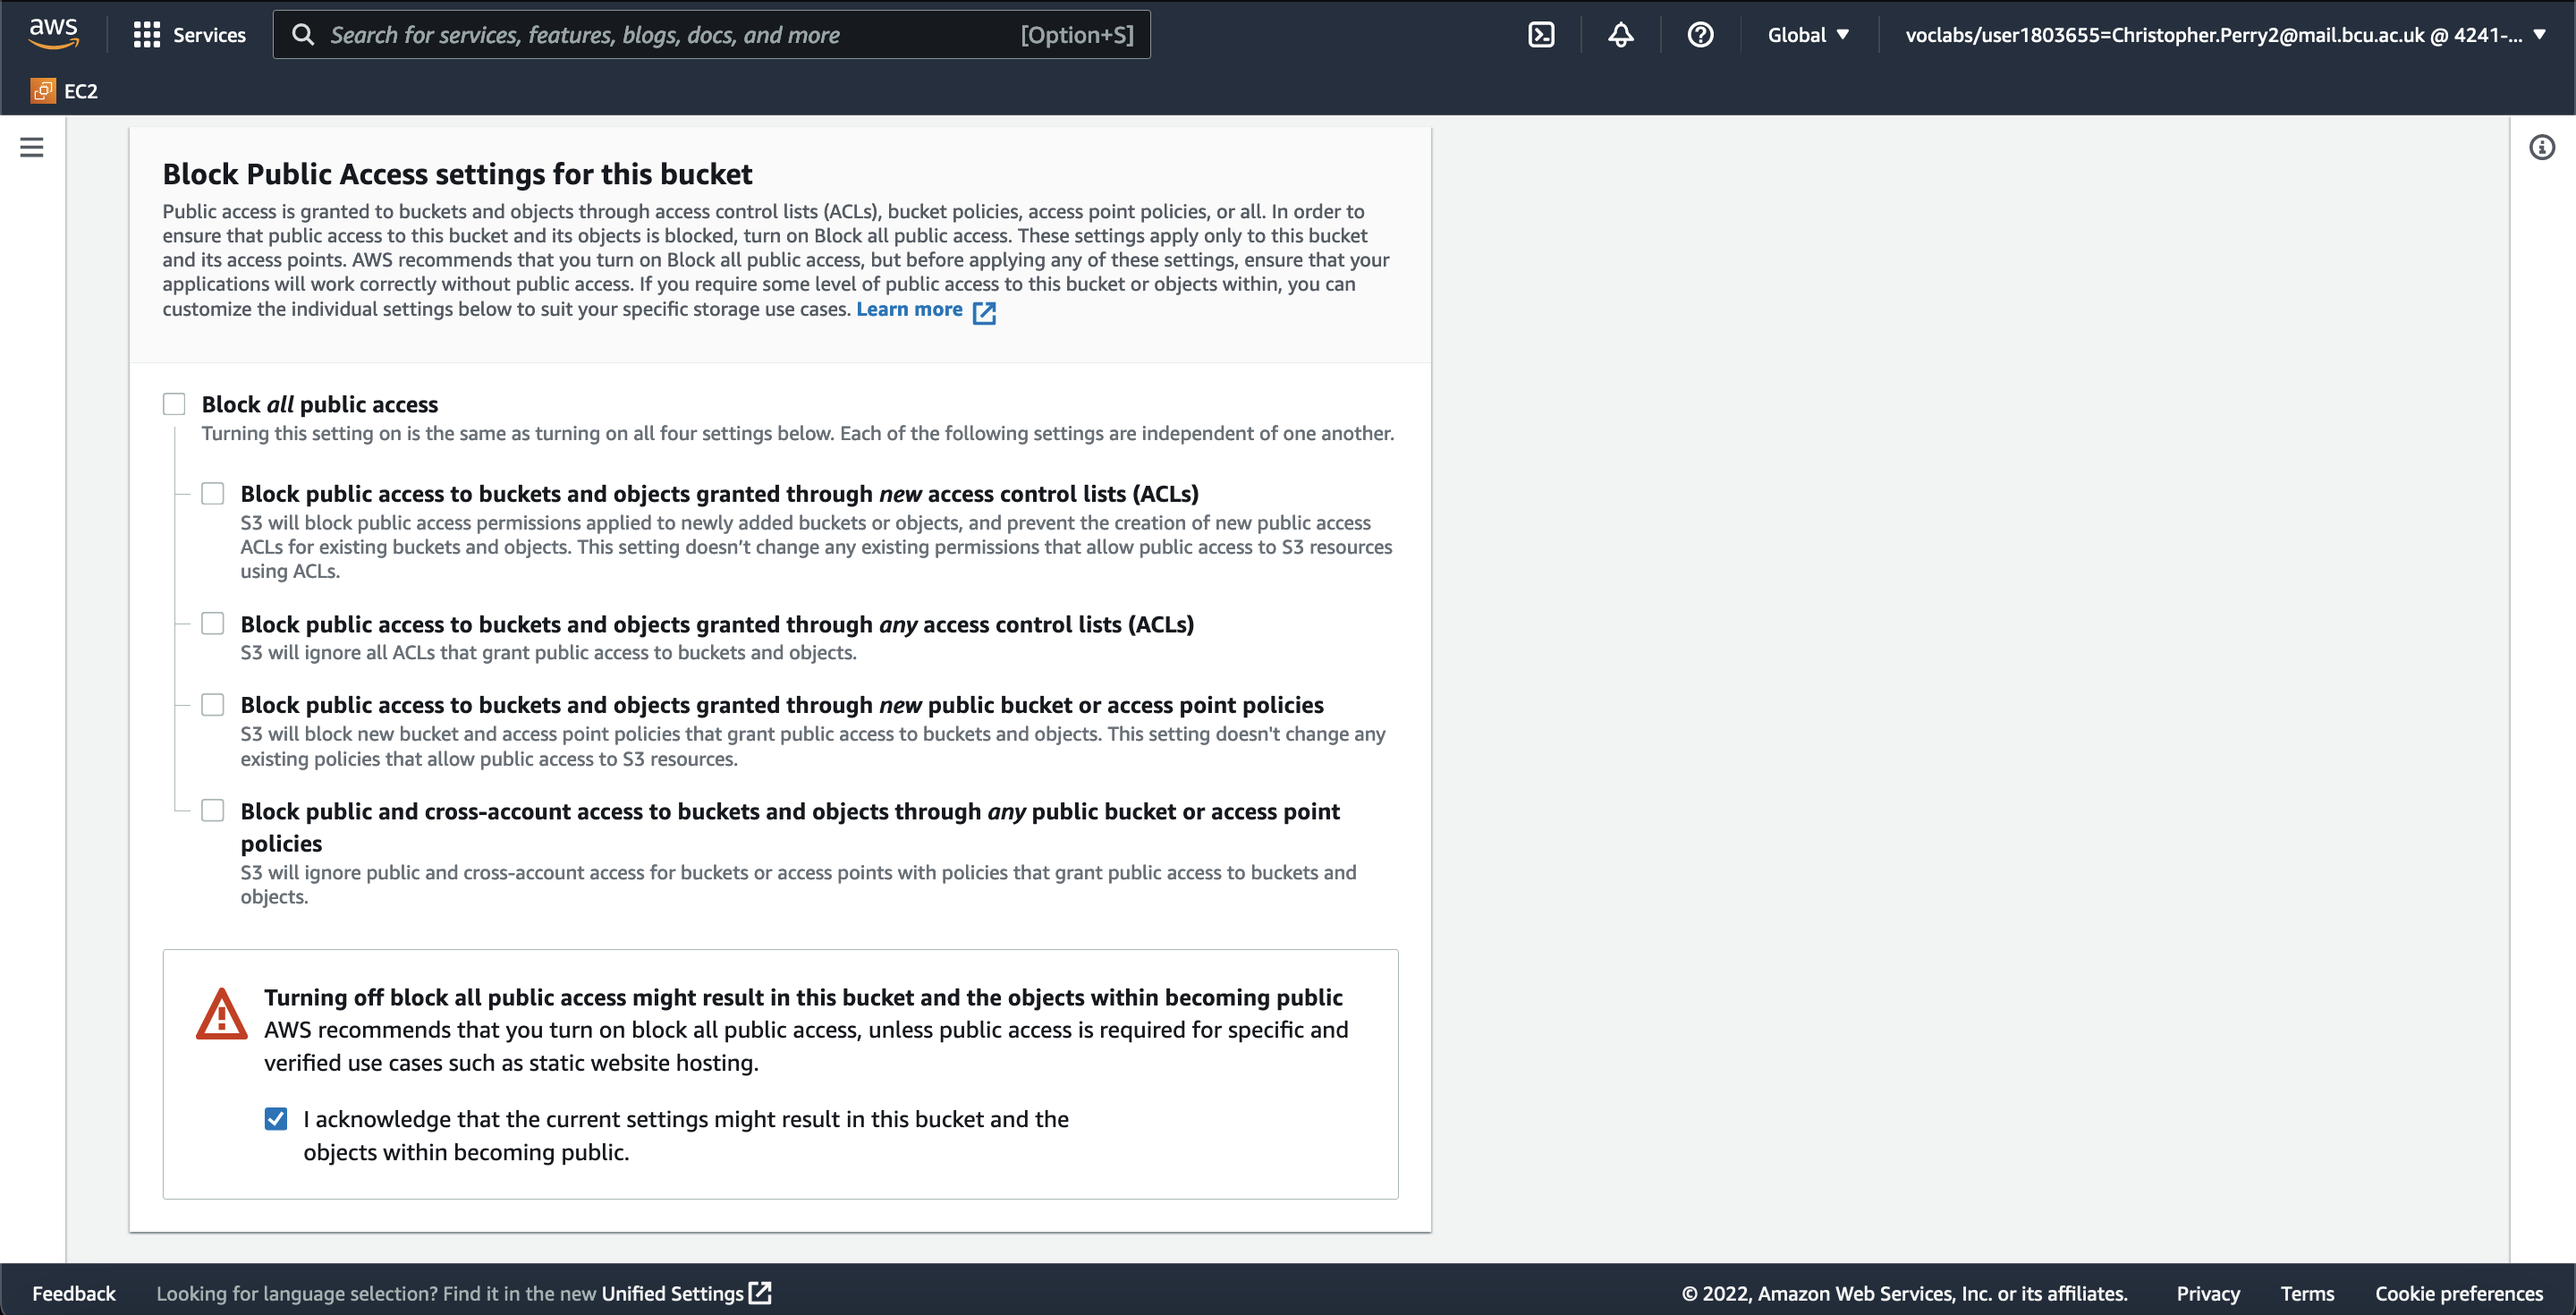
\includegraphics[width=125mm]{resources/s3/s3-public-access}
    \caption{Allowing public read access for images.}
    \label{fig:s3-public-access}
\end{figure}

After these configurations were set up, the S3 bucket was created with the name \mintinline{zsh}|group4-digital-ink-s3|.

\begin{figure}[!htbp]
    \centering
    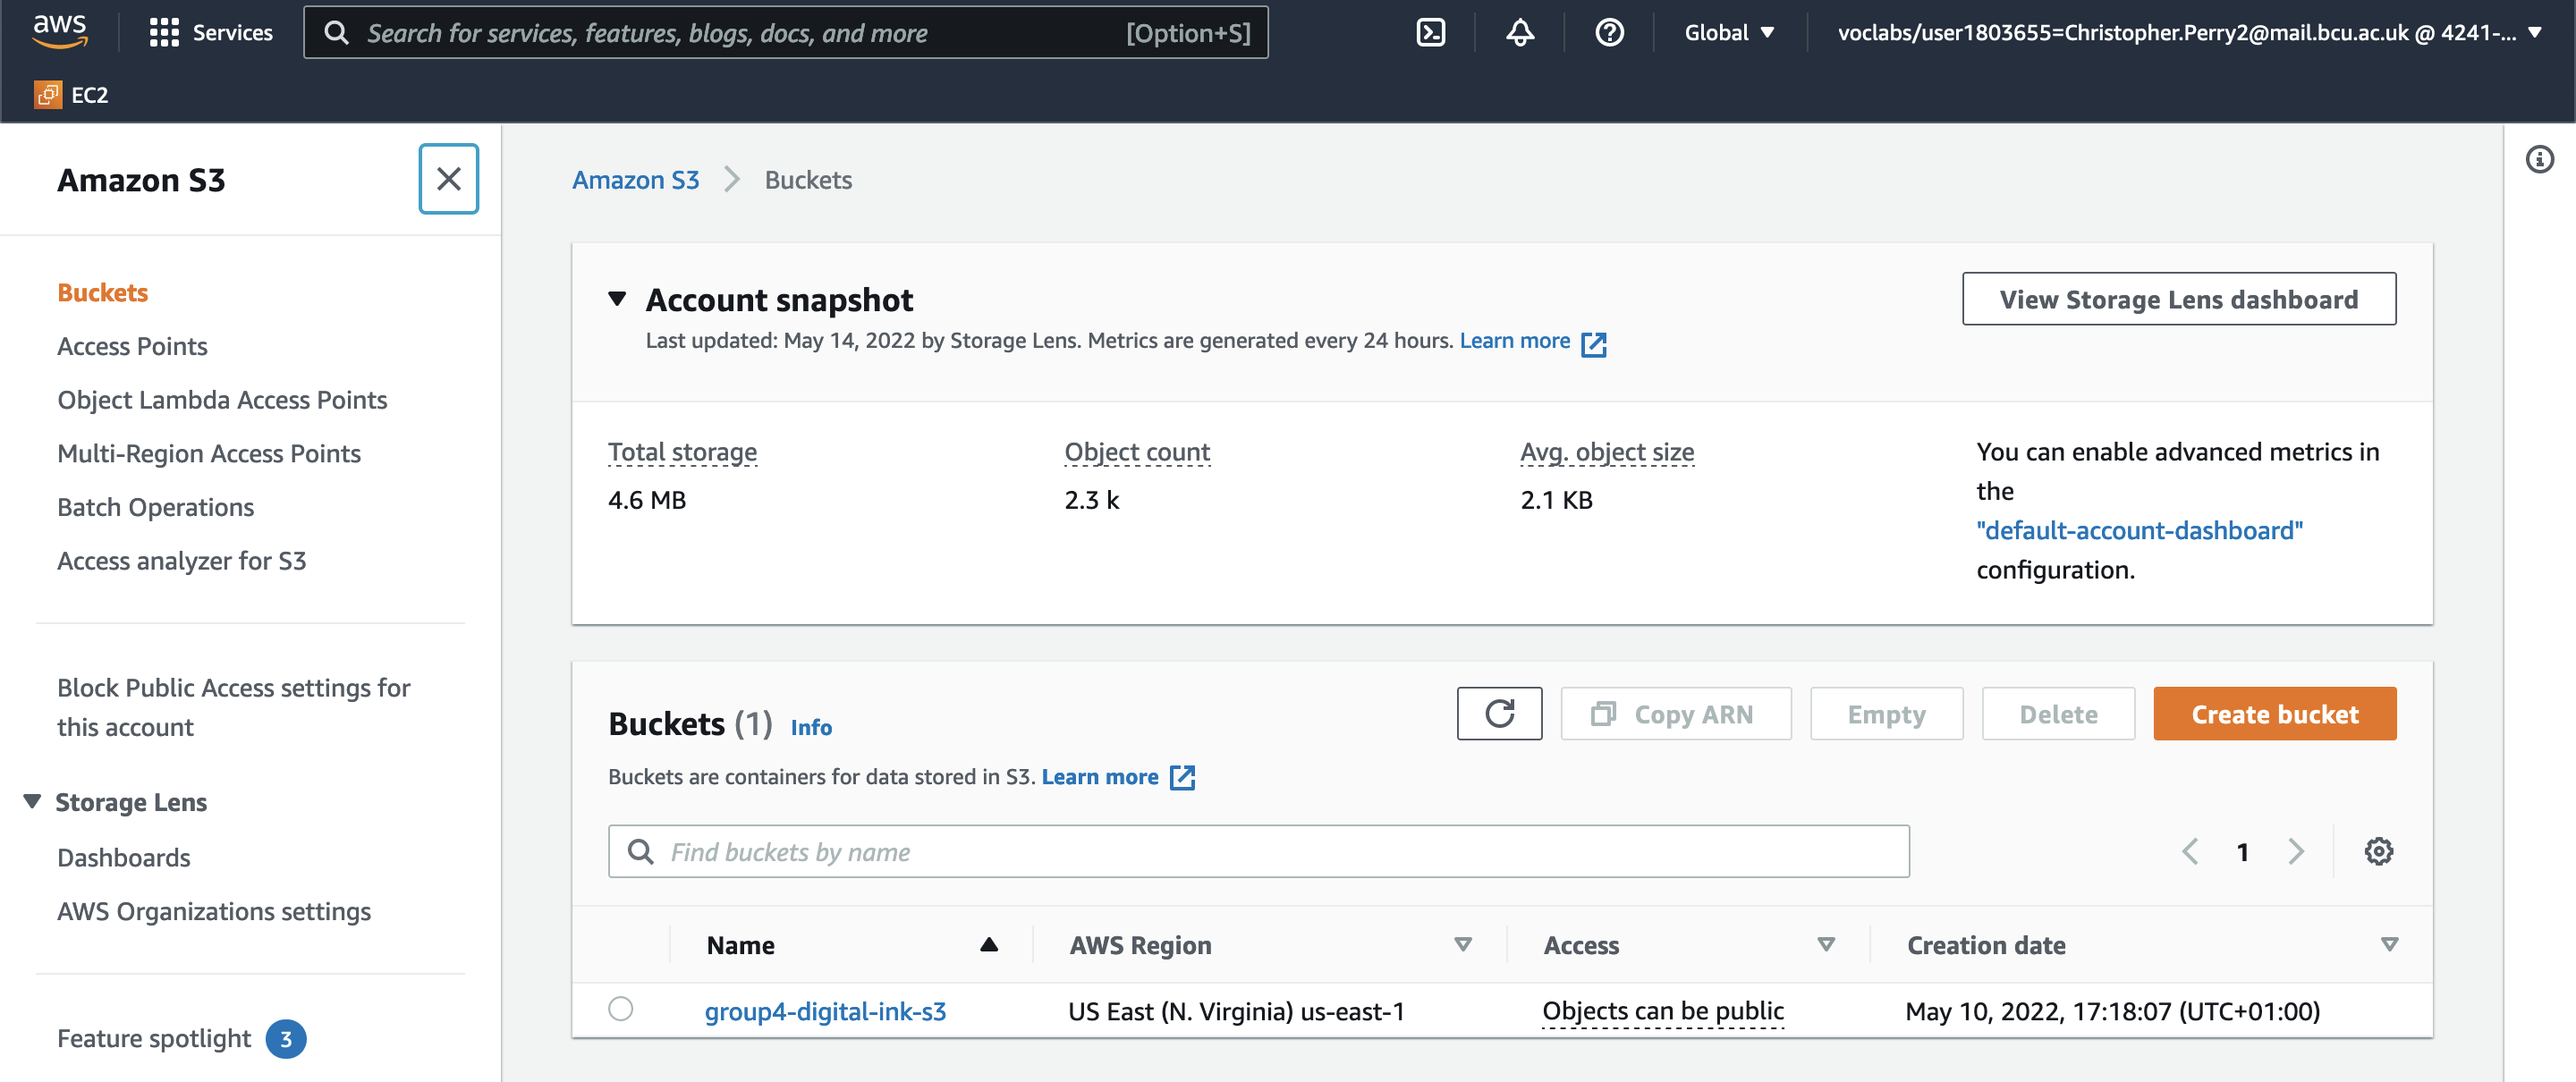
\includegraphics[width=125mm]{resources/s3/s3-created}
    \caption{Viewing the created S3 bucket.}
    \label{fig:s3-created}
\end{figure}

\pagebreak
\section{Utilising S3 URLs}
Now that the S3 bucket has been created to the needs of the web app, images must be uploaded to it.
Image files for the \textit{Digital-Ink} logo and external social media links were uploaded to the bucket.

\begin{figure}[!htbp]
    \centering
    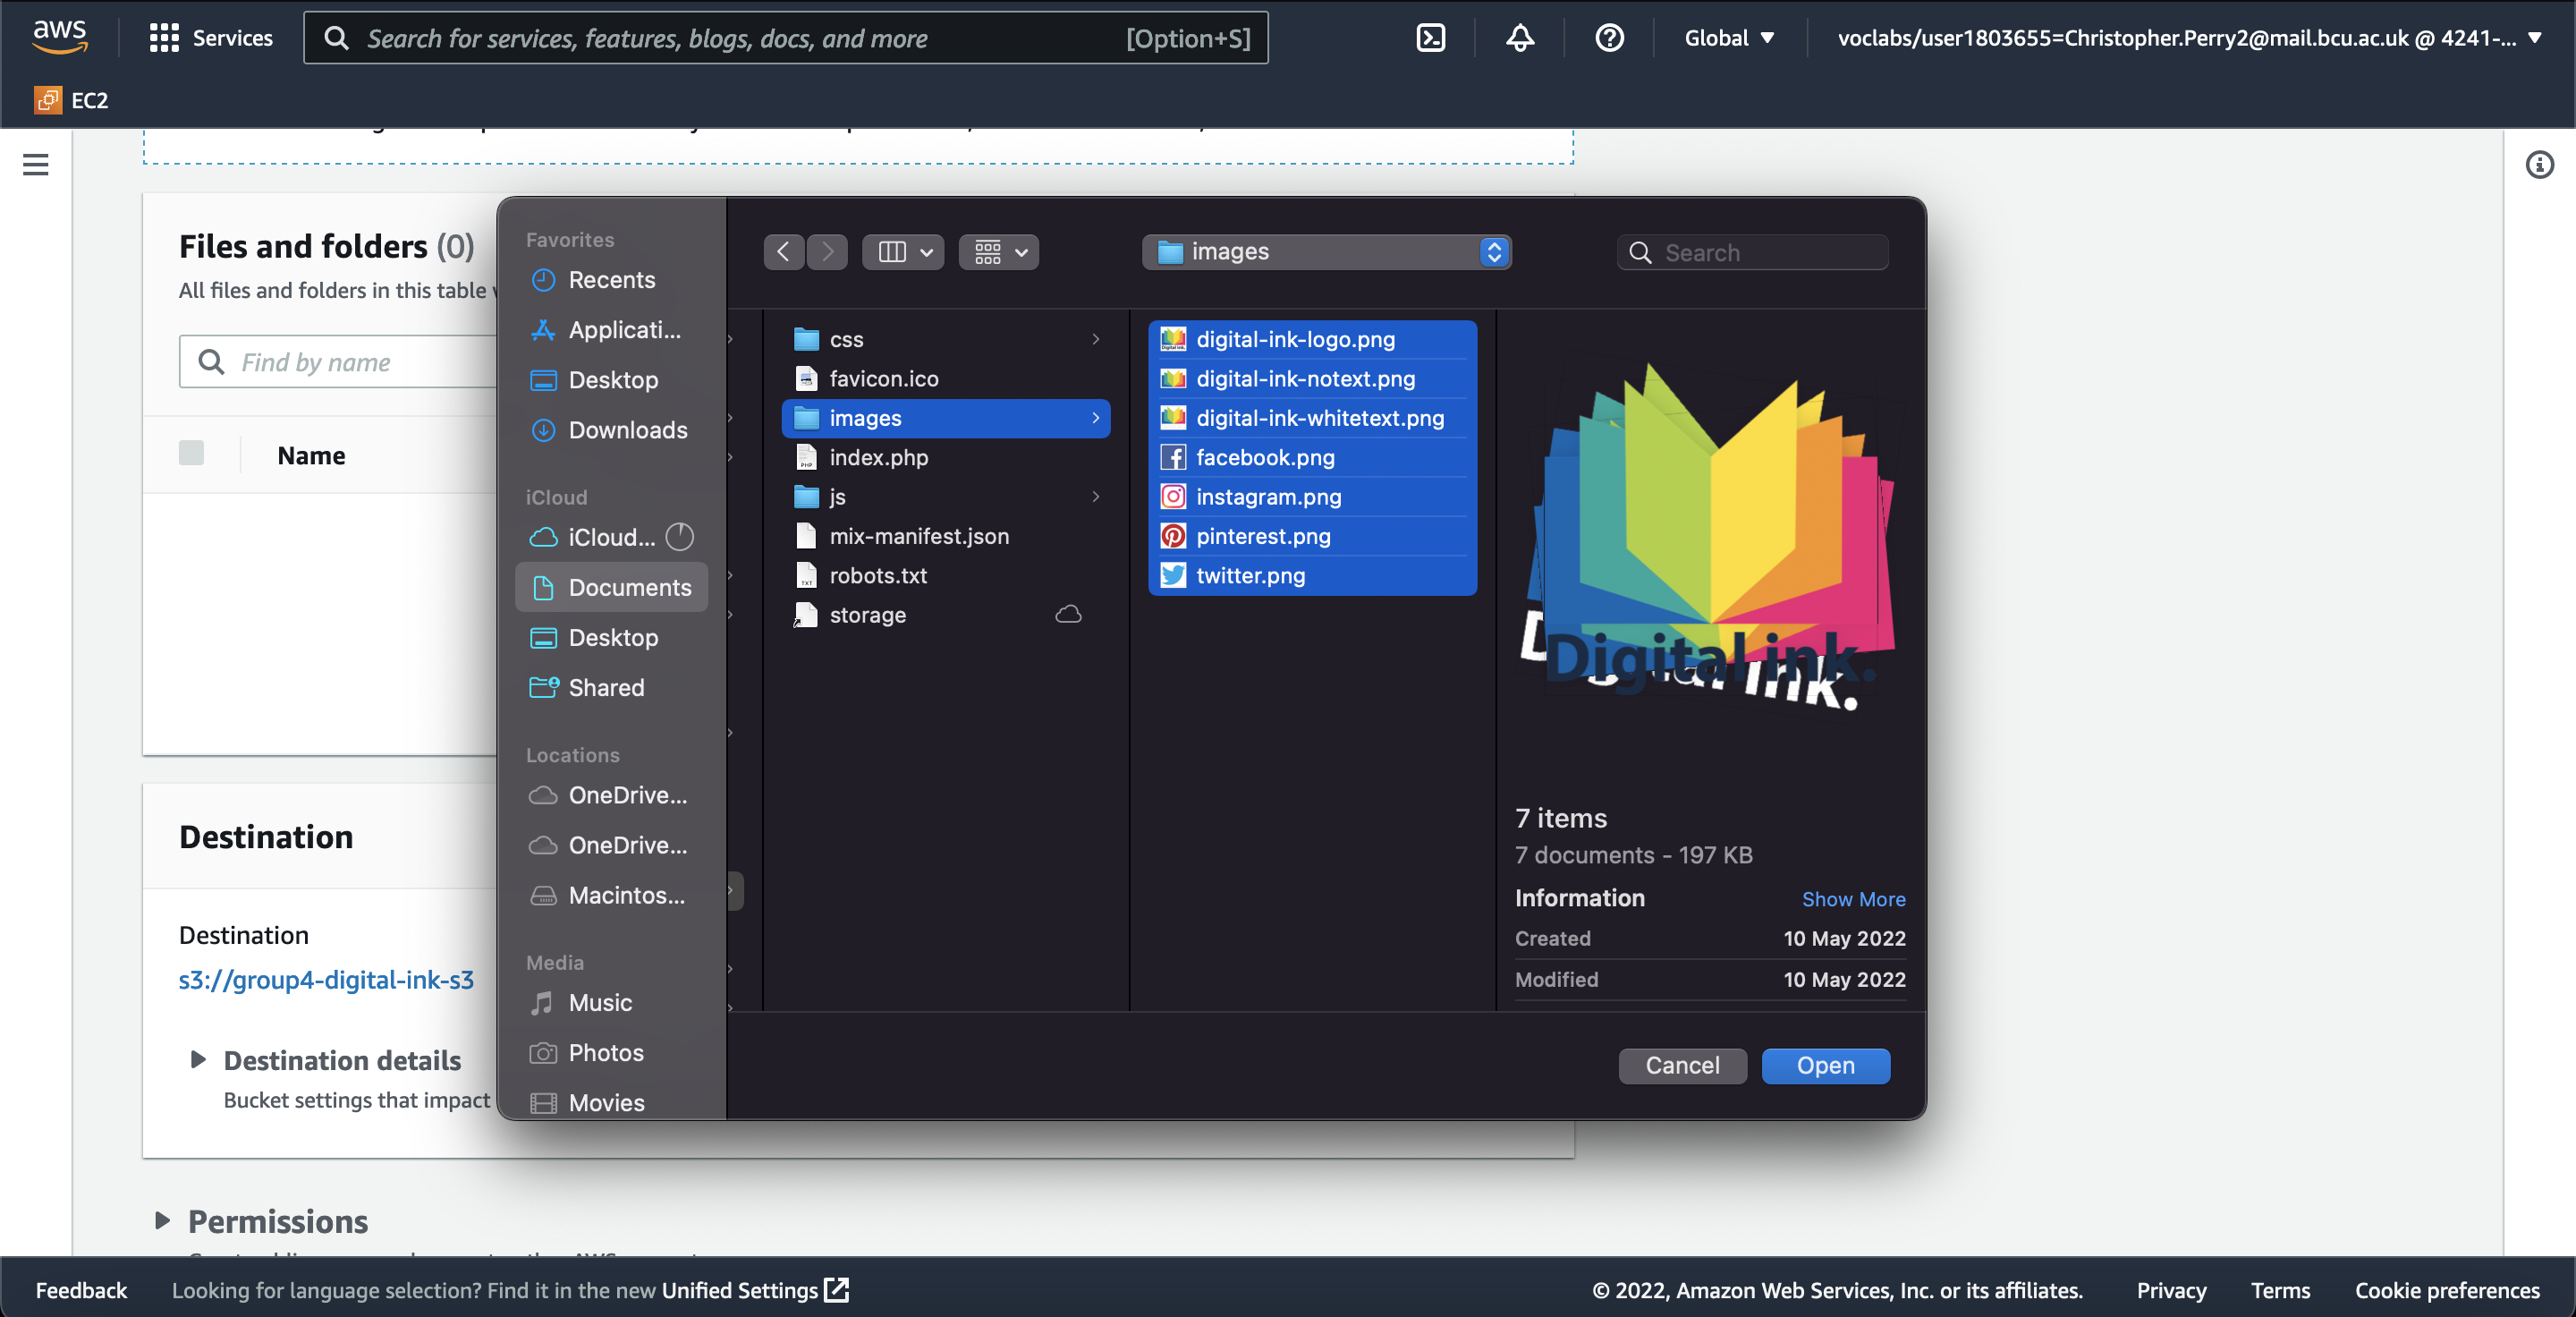
\includegraphics[width=\textwidth]{resources/s3/s3-image-upload}
    \caption{Uploading static image assets to the S3 bucket.}
    \label{fig:s3-image-upload}
\end{figure}

\begin{figure}[!htbp]
    \centering
    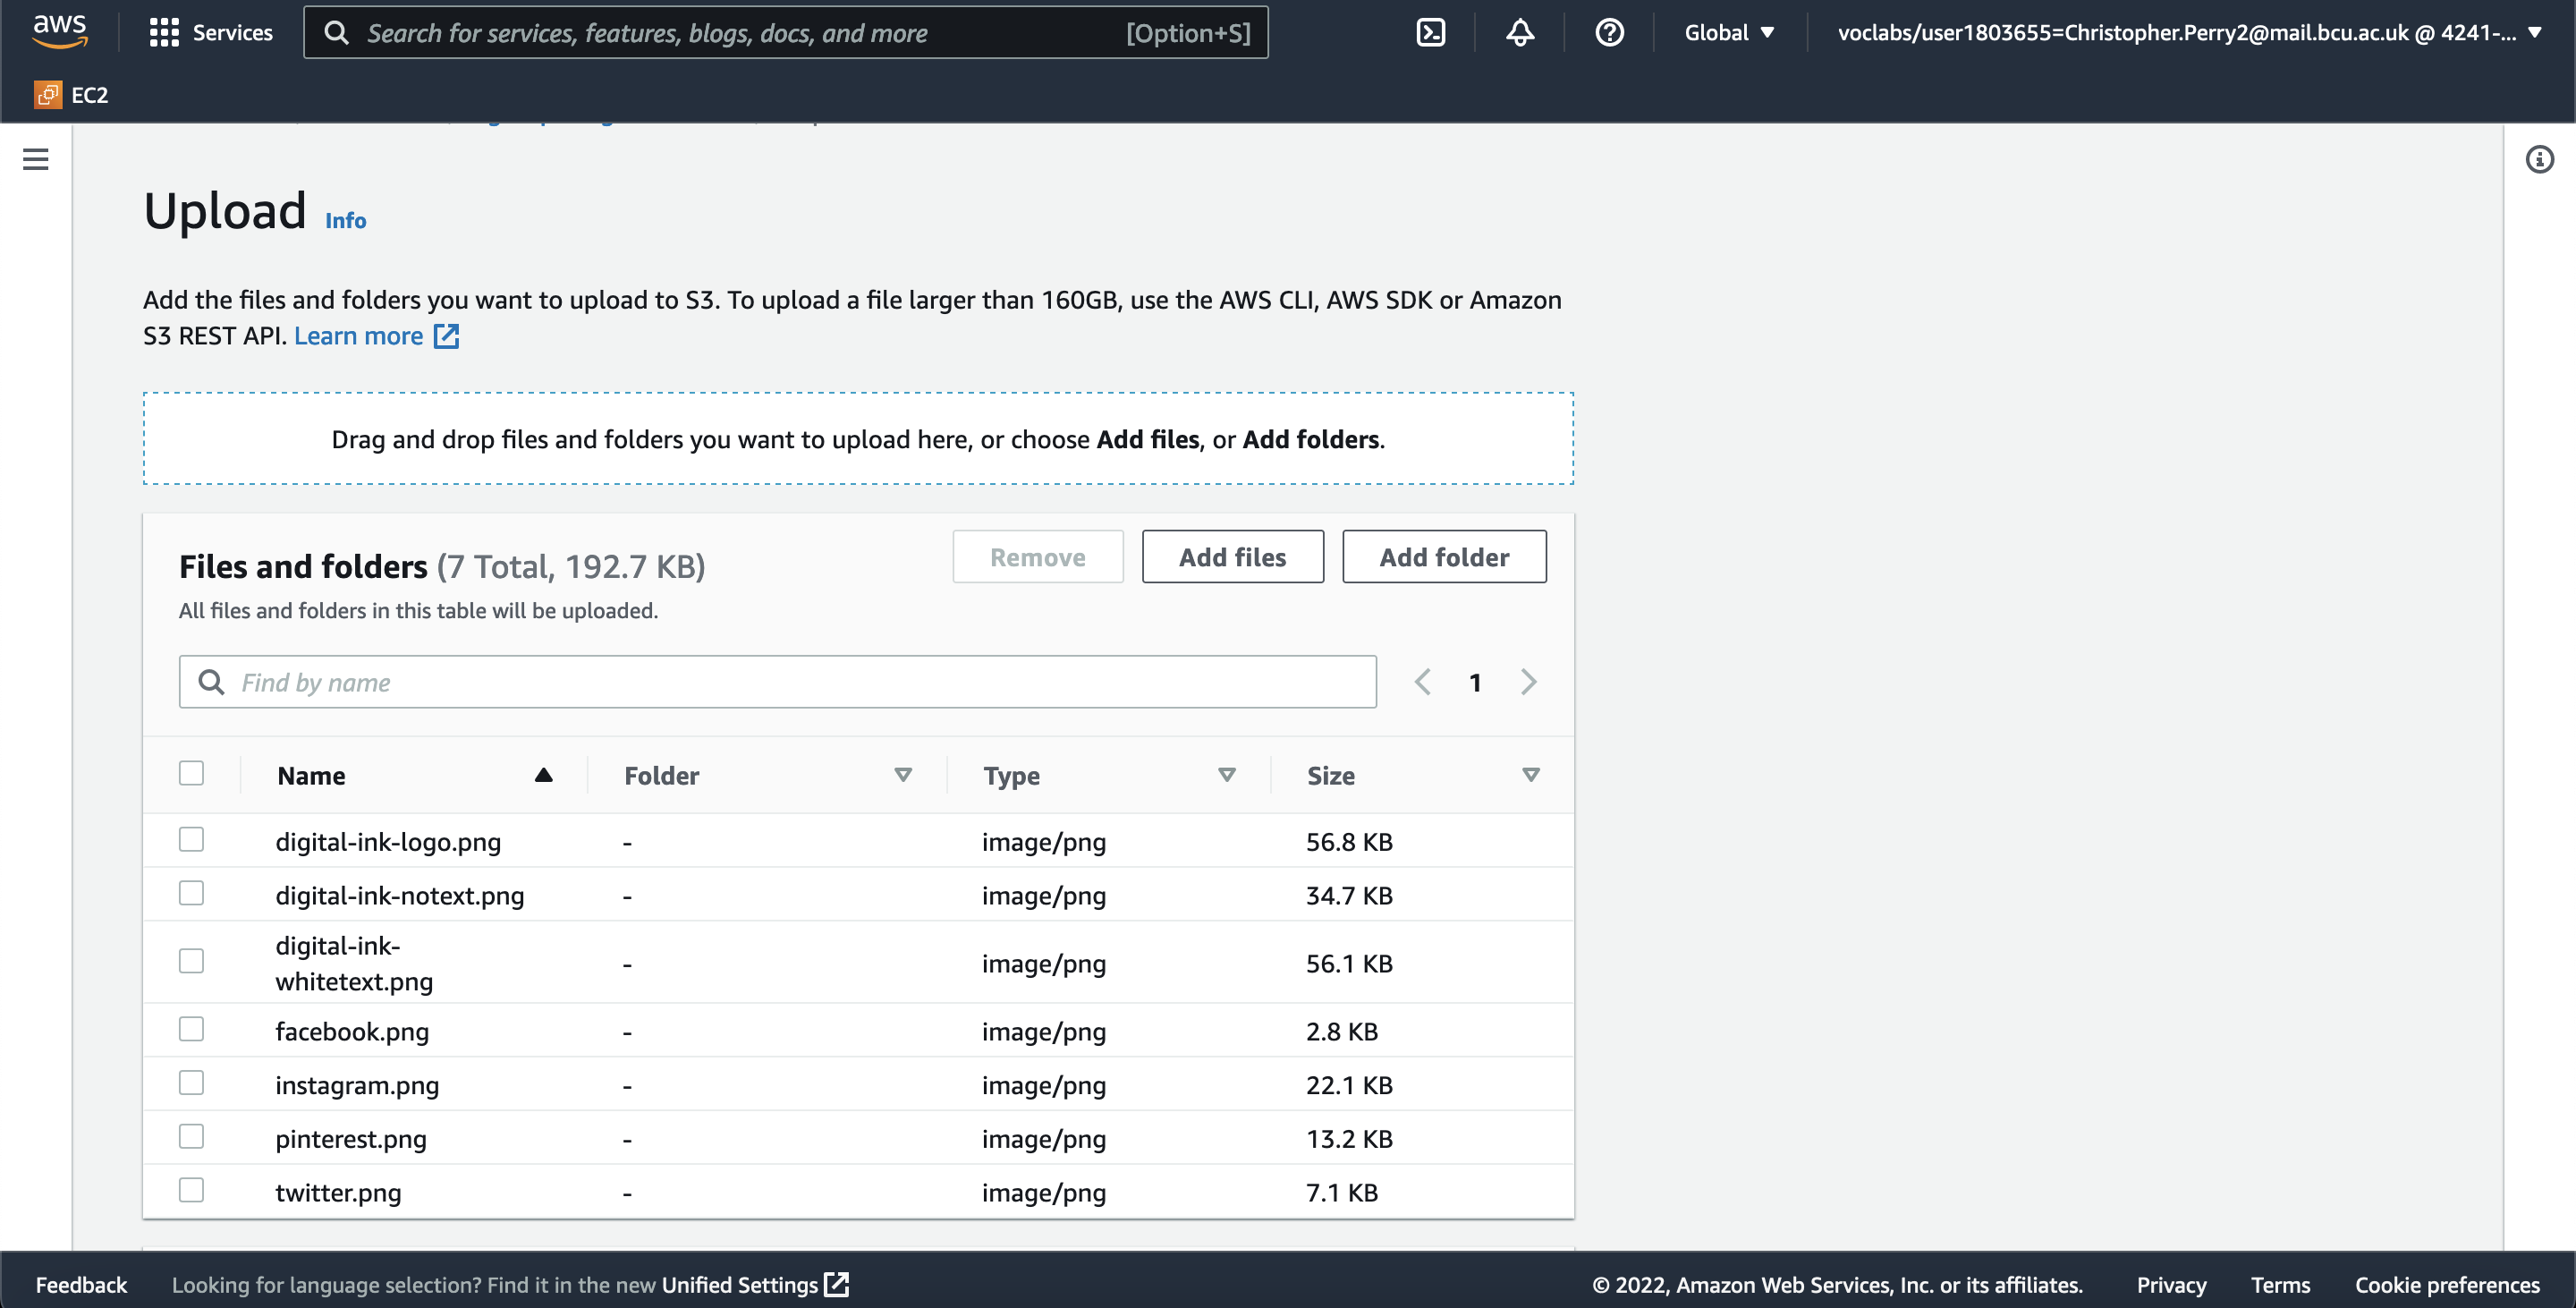
\includegraphics[width=\textwidth]{resources/s3/s3-upload-summary}
    \caption{Viewing the assets to be uploaded to the S3 bucket.}
    \label{fig:s3-upload-summary}
\end{figure}

\pagebreak
After the necessary files have been selected, they can be uploaded.
If no errors occur during this process, a message shows indicating success.
Once this has been done, all files attached to the bucket can be seen from the bucket page.

\begin{figure}[!htbp]
    \centering
    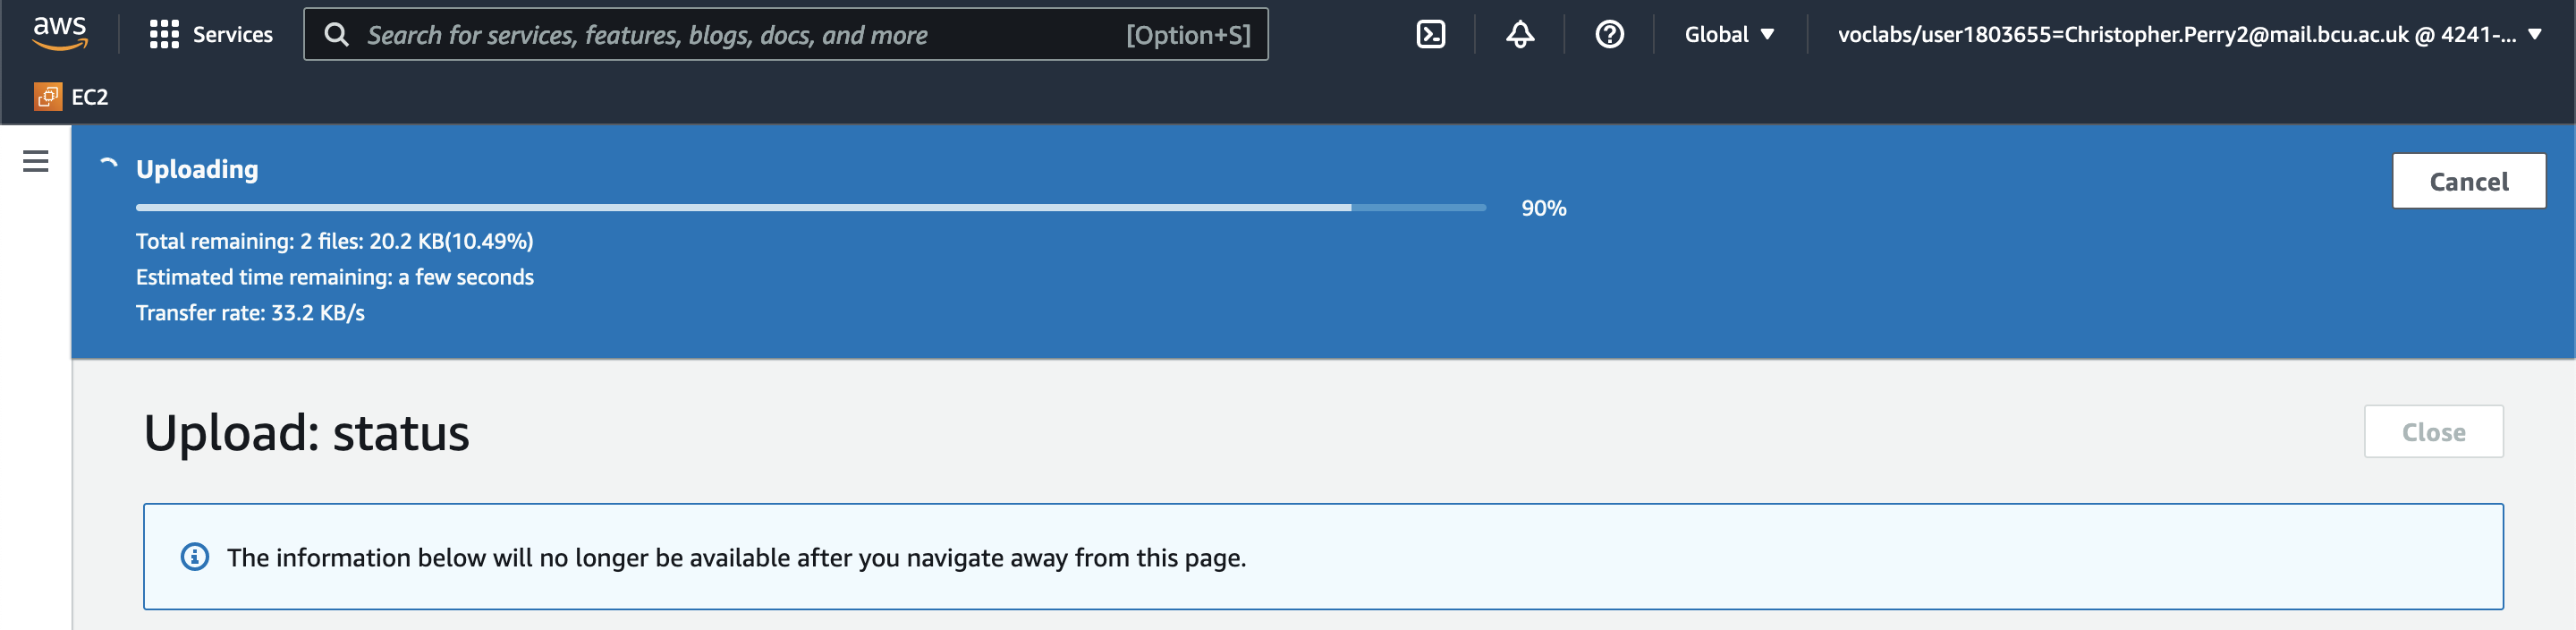
\includegraphics[width=\textwidth]{resources/s3/s3-uploading}
    \caption{S3 uploading in progress.}
    \label{fig:s3-uploading}
\end{figure}

\begin{figure}[!htbp]
    \centering
    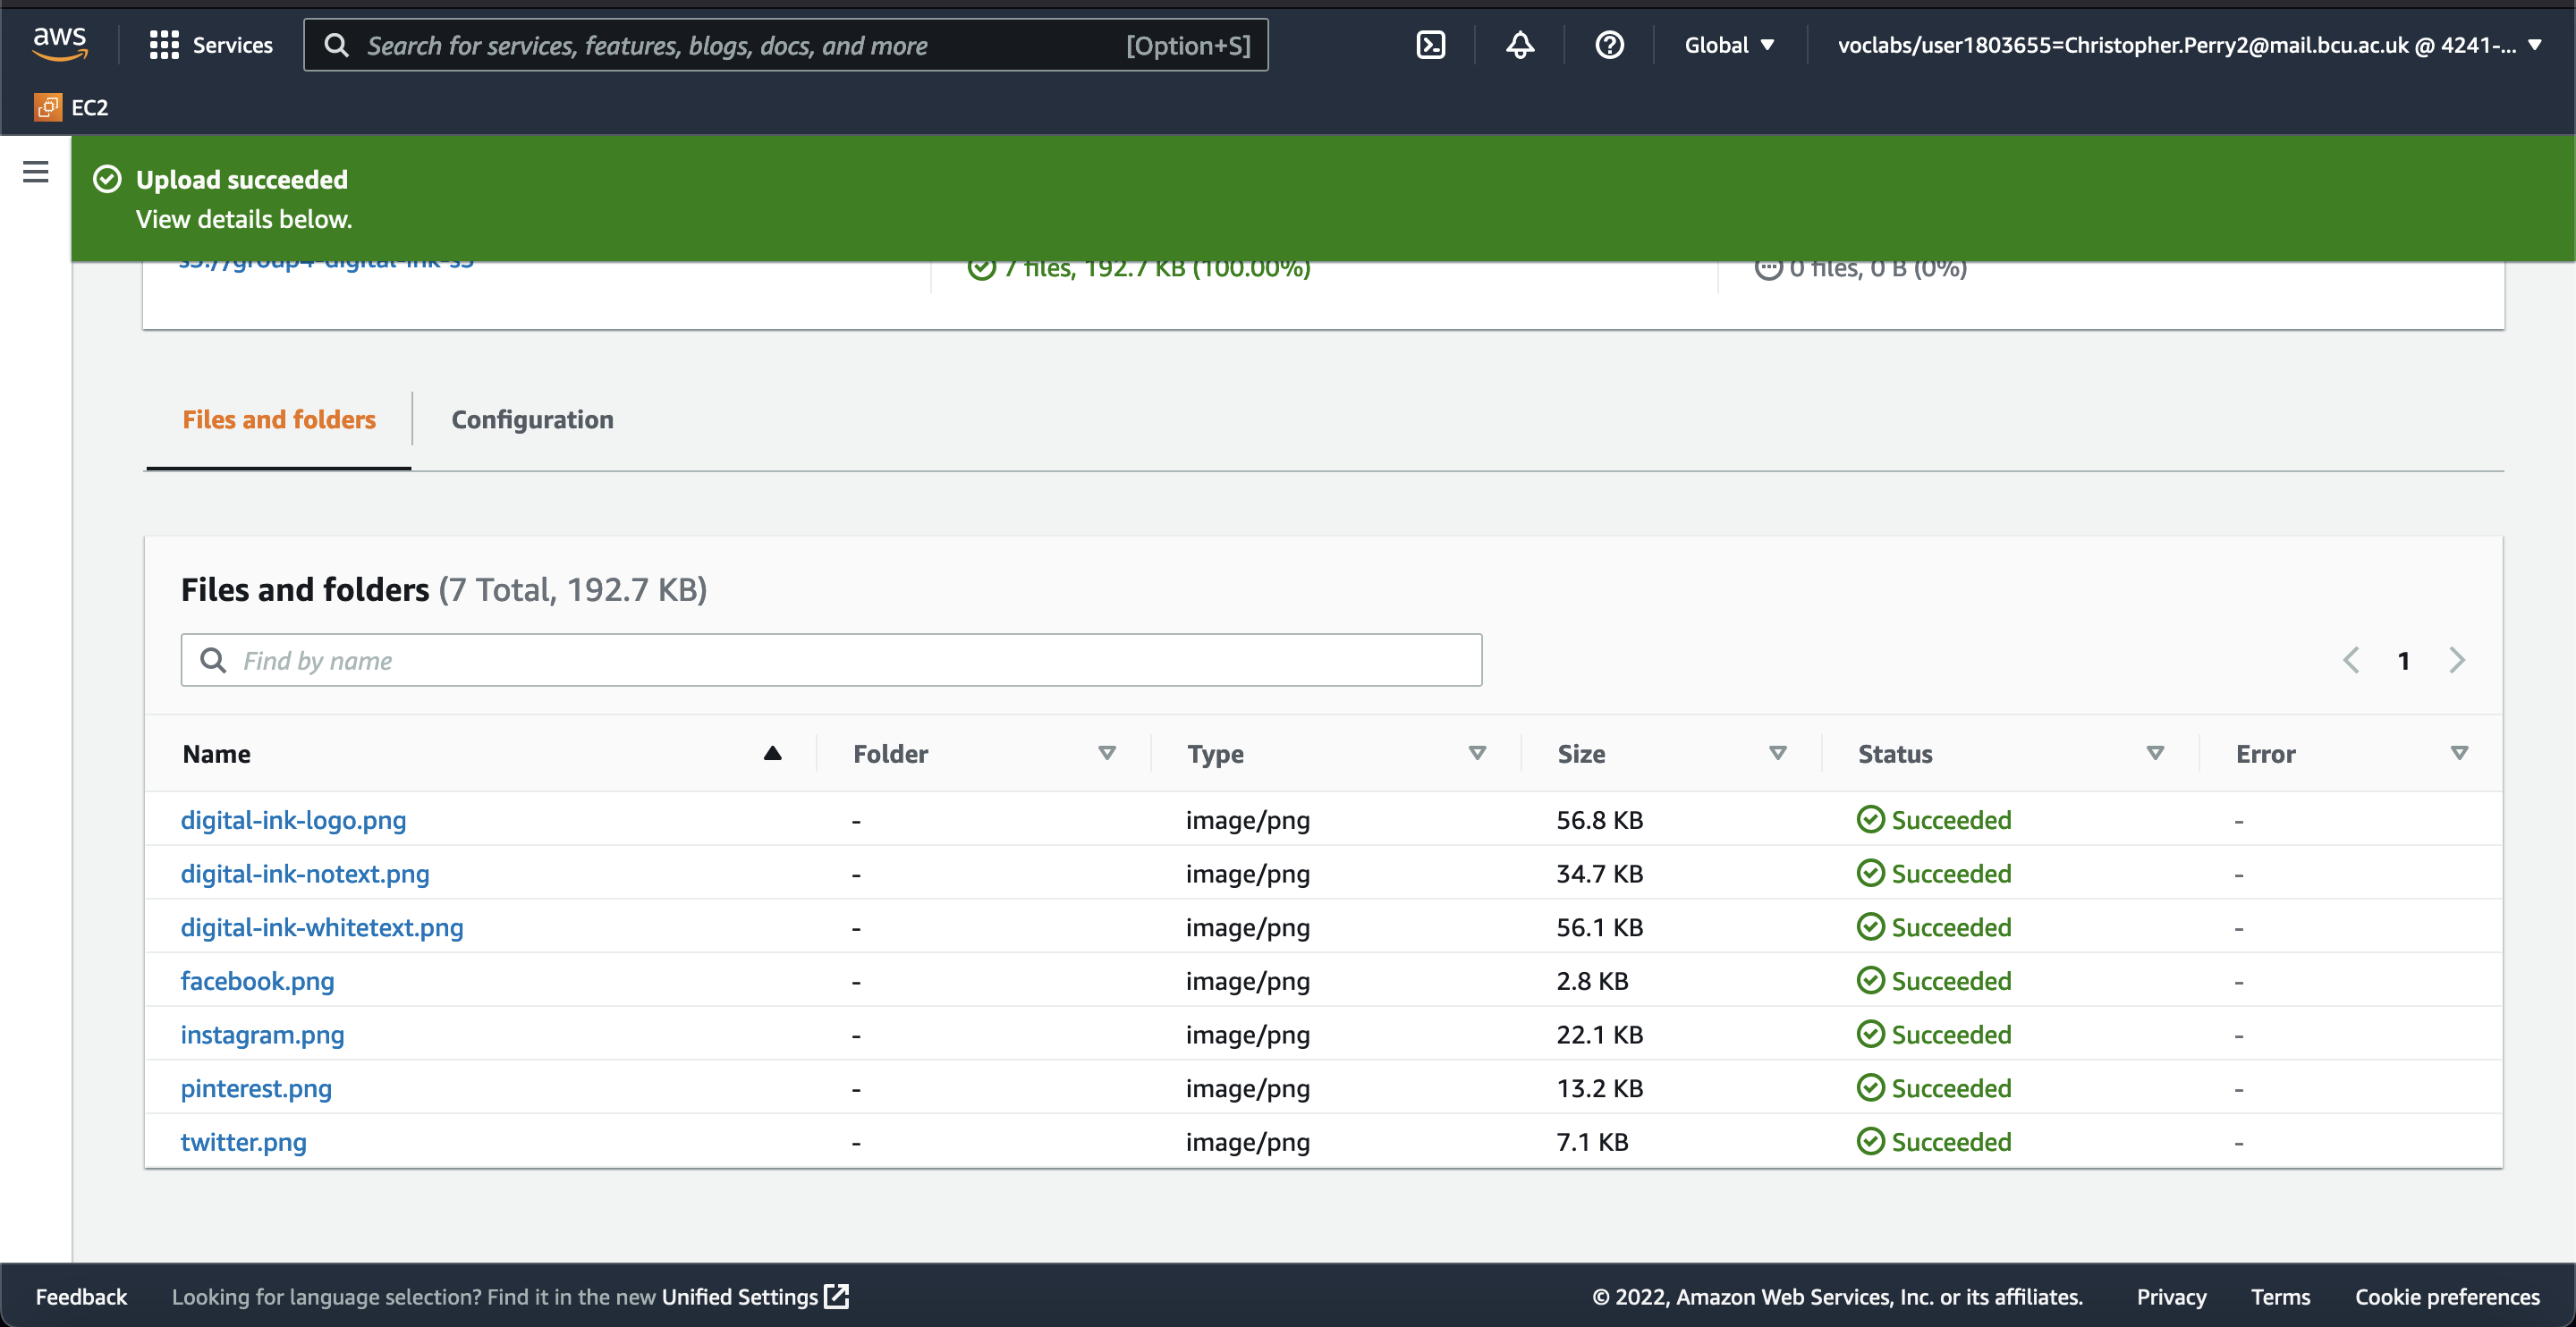
\includegraphics[width=\textwidth]{resources/s3/s3-uploaded}
    \caption{S3 successful upload and file summary.}
    \label{fig:s3-uploaded}
\end{figure}

\pagebreak
Now that images have been uploaded to the bucket, they can be used within the web app.
To do this, the asset image paths within the code of the web app must be changed to point to the S3 bucket
rather than the local storage.

\begin{figure}[!htbp]
    \centering
    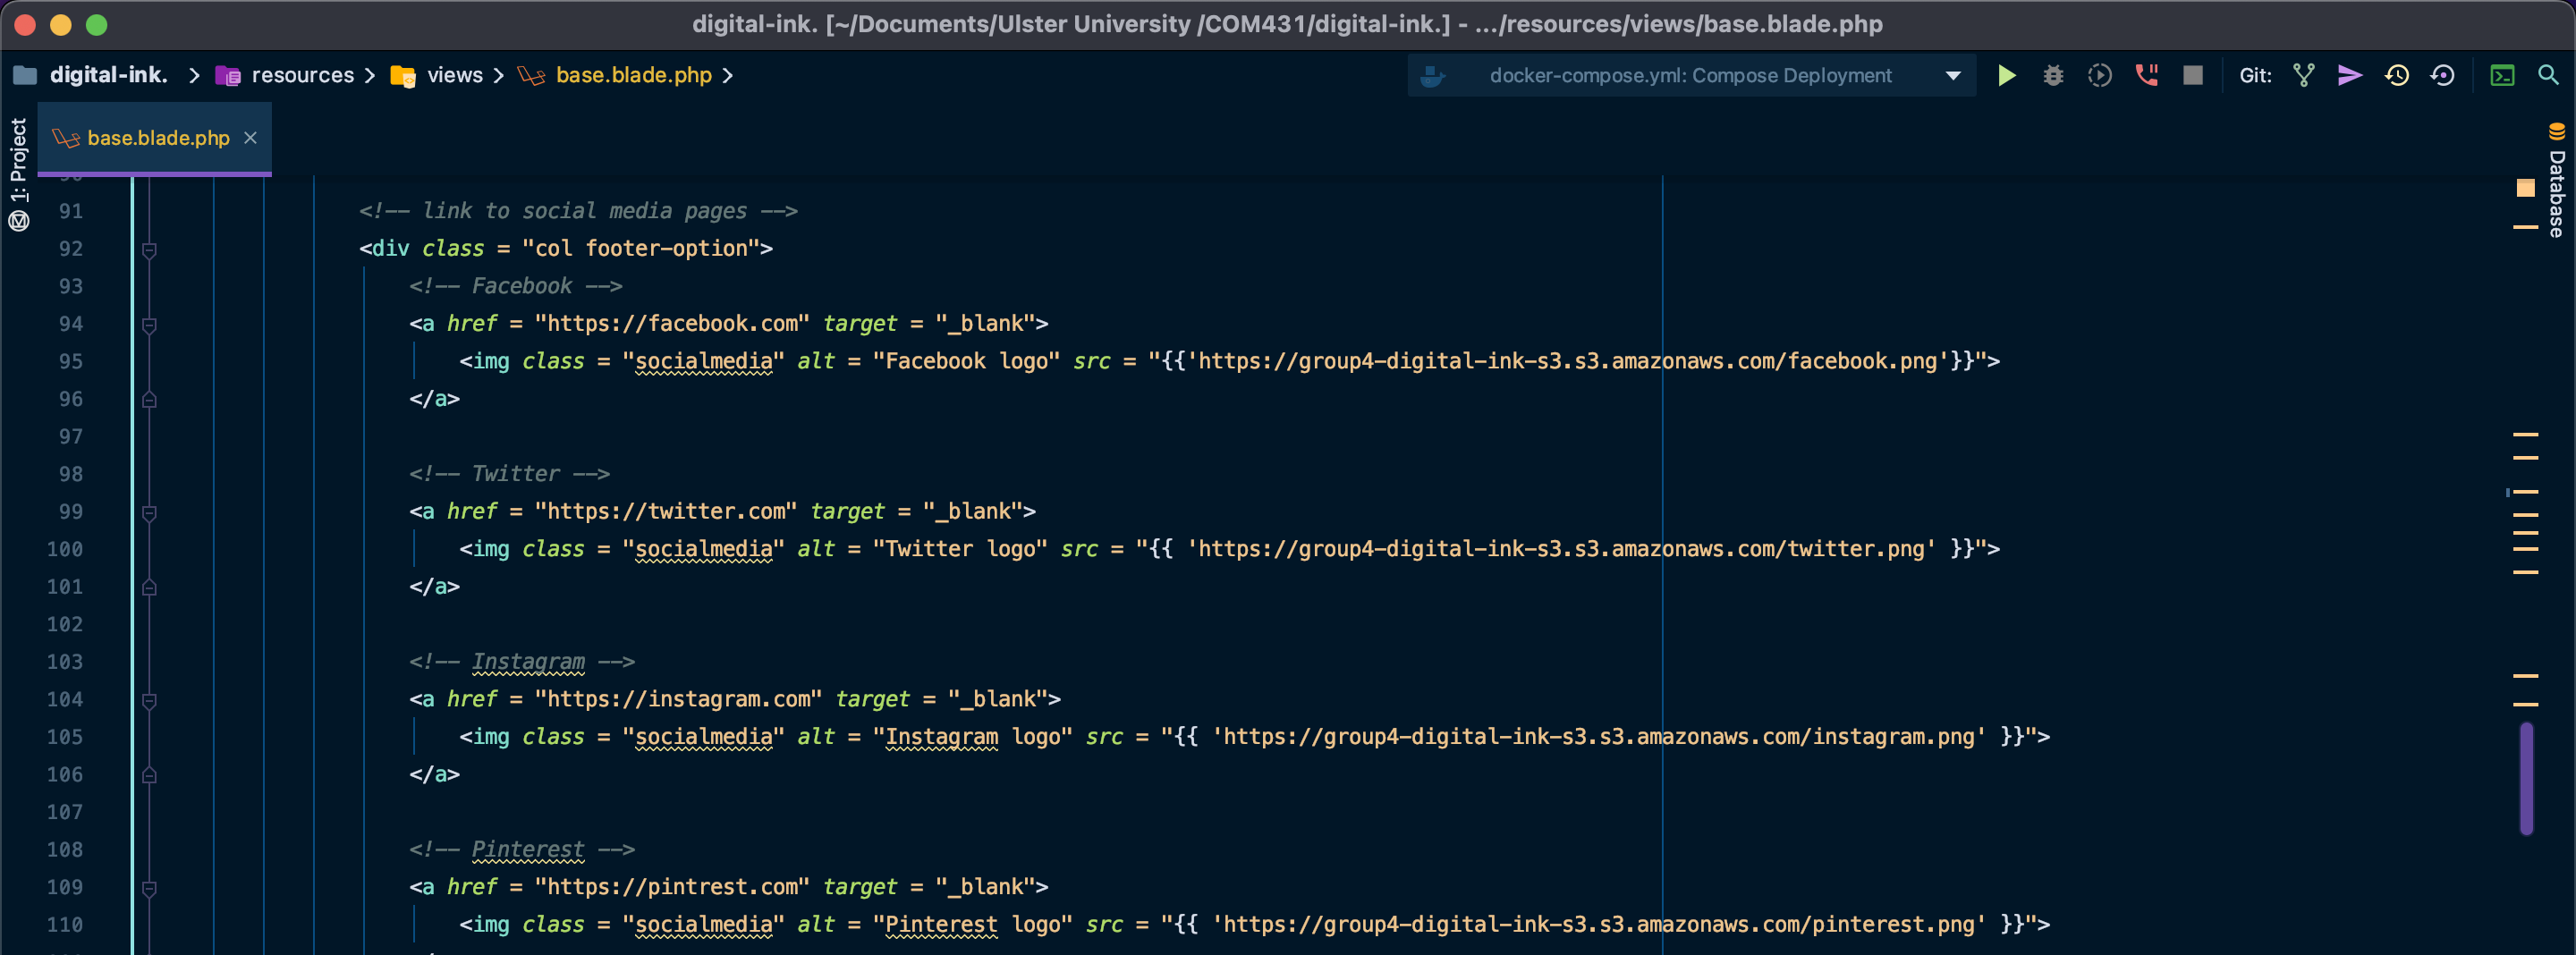
\includegraphics[width=\textwidth]{resources/s3/s3-url-change}
    \caption{Changing image paths within the web app code.}
    \label{fig:s3-url-change}
\end{figure}

To test that this use of S3 is working, the URL generated by the bucket which is hosting the image may be visited in a
browser for confirmation.

\begin{figure}[!htbp]
    \centering
    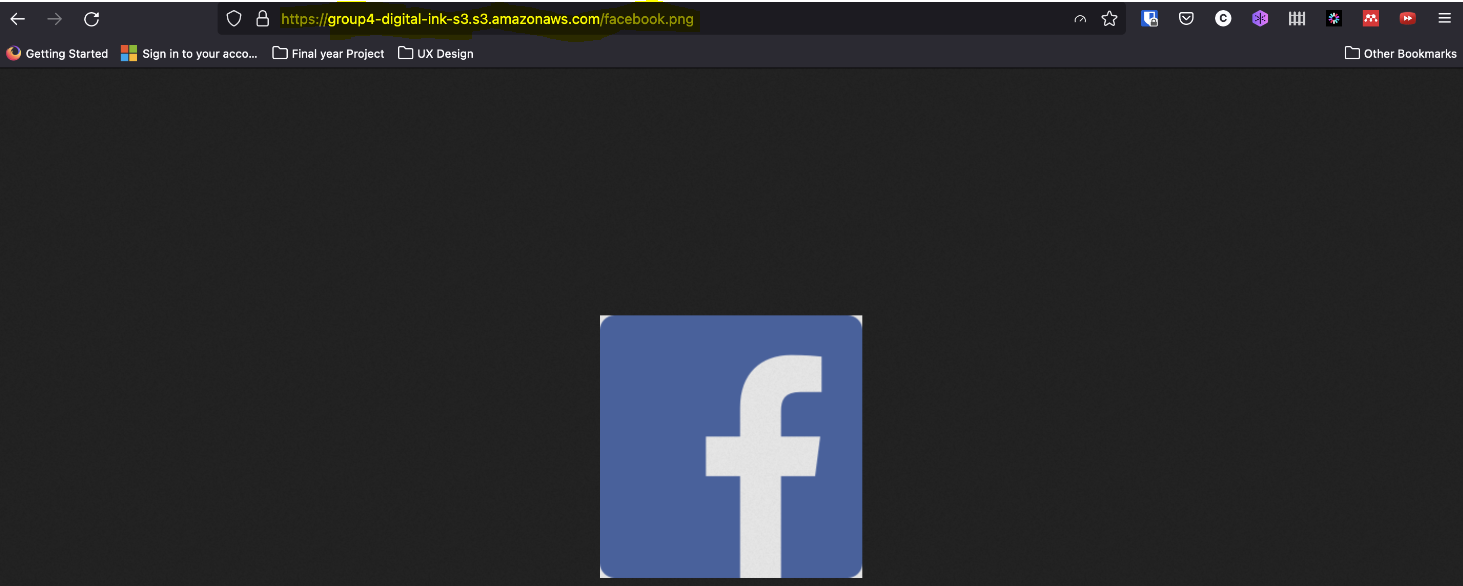
\includegraphics[width=\textwidth]{resources/s3/s3-image-displayed}
    \caption{Accessing an image using the S3 bucket URL.}
    \label{fig:s3-image}
\end{figure}
